%%%%%%%%%%%%%%%%%%%%%%%%%%%%%%%%%%%%%%%%%
% Focus Beamer Presentation
% LaTeX Template
% Version 1.0 (8/8/18)
%
% This template has been downloaded from:
% http://www.LaTeXTemplates.com
%
% Original author:
% Pasquale Africa (https://github.com/elauksap/focus-beamertheme) with modifications by
% Vel (vel@LaTeXTemplates.com)
%
% Template license:
% GNU GPL v3.0 License
%
% Important note:
% The bibliography/references need to be compiled with bibtex.
%
%%%%%%%%%%%%%%%%%%%%%%%%%%%%%%%%%%%%%%%%%

%----------------------------------------------------------------------------------------
%	PACKAGES AND OTHER DOCUMENT CONFIGURATIONS
%----------------------------------------------------------------------------------------

\documentclass{beamer}

\usetheme{focus} % Use the Focus theme supplied with the template
% Add option [numbering=none] to disable the footer progress bar
% Add option [numbering=fullbar] to show the footer progress bar as always full with a slide count

% Uncomment to enable the ice-blue theme
%\definecolor{main}{RGB}{92, 138, 168}
%\definecolor{background}{RGB}{240, 247, 255}

%------------------------------------------------

\usepackage[french]{babel}
\usepackage{booktabs} % Required for better table rules
\usepackage{csquotes}
\usepackage{emoji}
\usepackage{enumitem}
\usepackage{hyperref}
\usepackage{minted}
\usepackage[T1]{fontenc}
\usepackage{svg} % to access the named colour LightGray
\usepackage{xcolor} % to access the named colour LightGray
\definecolor{LightGray}{gray}{0.9}

\hypersetup{
    pdfborderstyle={/S/U/W 1}
}


\AtBeginSection[]
{\begin{frame}
    \frametitle{Sommaire}
    \tableofcontents[currentsection]
\end{frame}
}
%----------------------------------------------------------------------------------------
%	 TITLE SLIDE
%----------------------------------------------------------------------------------------

\title{La délivrabilité e-mail}

\subtitle{SPF, DKIM, DMARC, ??}

\author{\href{mailto:mail@franek.fr}{François FREITAG}}

\titlegraphic{\vspace{25pt} \frame{
\includegraphics[scale=0.22]{Images/Spam.jpg}}}

\institute{Les emplois de l'inclusion \\ GIP Inclusion}

\date{9 septembre 2024}

%------------------------------------------------

\begin{document}

%------------------------------------------------

\begin{frame}
	\maketitle % Automatically created using the information in the commands above
\end{frame}

%----------------------------------------------------------------------------------------
%	 SECTION 1
%----------------------------------------------------------------------------------------

\section{E-mail} % Section title slide, unnumbered

\begin{frame}[fragile]
    \frametitle{\href{https://datatracker.ietf.org/doc/html/rfc5322}{Anatomie d'un e-mail - RFC 5322}}

    \begin{minted}[bgcolor=LightGray]{text}
Date: Tue, 3 Sep 2024 11:11:11 +0200
From: The Sender <sender@email.test>
To: me@beta.gouv.fr
Message-ID: <430617367.736715.1725348550243@uniq>
Subject: Mon message pour vous
Content-Type: text/plain; charset=UTF-8
Content-Transfer-Encoding: 8bit
Return-Path: <me@beta.gouv.fr>

Salutations de rigueur,

Le corps de l'email.

--
Moi
    \end{minted}
\end{frame}

\begin{frame}{La circulation des emails}
    \begin{figure}[b]
        \includesvg[height=.4\textheight]{Images/SMTP_transfer_model.svg}
        \caption{source: \href{https://commons.wikimedia.org/wiki/File:SMTP-transfer-model.svg}{https://commons.wikimedia.org/wiki/File:SMTP-transfer-model.svg}}
        % Ale2006-from-en, CC BY-SA 3.0 <https://creativecommons.org/licenses/by-sa/3.0>, via Wikimedia Commons
    \end{figure}

    \begin{description}
        \item[MUA] Mail User Agent
        \item[MSA] Mail Submission Agent
        \item[MTA] Mail Transfer Agent (Mail Relay)
        \item[MDA] Mail Delivery Agent
    \end{description}
\end{frame}

\begin{frame}[fragile]
    \frametitle{MX : Mail eXchanger}
    Ensemble d'entrées DNS pour un domaine indiquant quels serveurs e-mail contacter, avec un ordre de priorité :
    \begin{minted}[bgcolor=LightGray,fontsize=\footnotesize]{text}
example.org.       MX      10 principal.example.org.
                   MX      50 secondaire.example.org.
    \end{minted}
\end{frame}

\begin{frame}[fragile]
    \frametitle{Simple Mail Transfer Protocol}

    \begin{minted}[bgcolor=LightGray,fontsize=\scriptsize]{text}
> telnet smtp.----.---- 25
< Connected to smtp.----.----.
< 220 smtp.----.---- SMTP Ready
> HELO yyyy.yyyy
< 250-smtp.----.----
< 250-PIPELINING
< 250 8BITMIME
> MAIL FROM: <auteur@yyyy.yyyy>
< 250 Sender ok
> RCPT TO: <destinataire@----.---->
< 250 Recipient ok.
> DATA
< 354 Enter mail, end with "." on a line by itself
> Subject: Test
>
> Corps du texte
> .
< 250 Ok
> QUIT
< 221 Closing connection
Connection closed by foreign host.
    \end{minted}
\end{frame}

\section{Spam}

\begin{frame}{Histoire du spam}
    \begin{description}
        \item[1978] : Email de publicité de Digital Equipment Corporation sur ARPANET par un membre du marketing
        \item[1993] : Accidentellement posté 200 messages sur Usenet, première utilisation du terme spam
        \item[1994] : Deux avocats (Canter \& Siegel) embauchent un dev pour "spammer" (5 500 messages) Usenet avec une pub pour la lotterie pour l'obtention d'une green card. \\
            \Rightarrow \$100-200K
    \end{description}
\end{frame}

\begin{frame}{Premier spam à succès}
    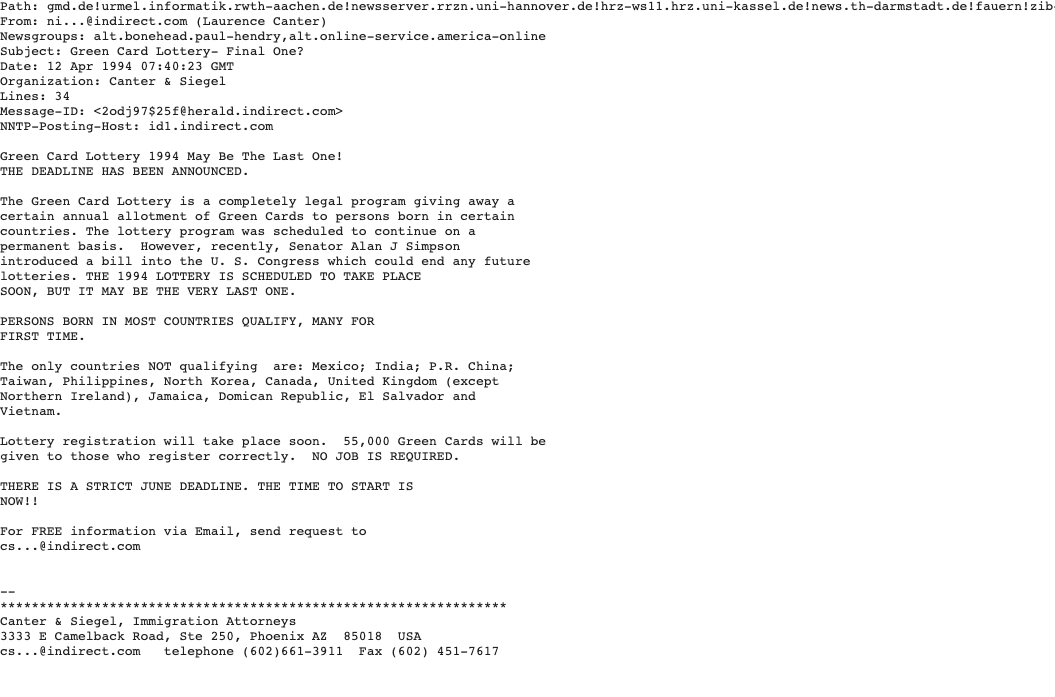
\includegraphics[width=.8\textwidth]{Images/spam.png}
\end{frame}

\begin{frame}{Le nom spam}
    \href{https://youtu.be/ycKNt0MhTkk?feature=shared&t=147}{Un sketch des Monty Python} \\

    
\includegraphics[width=.6\textwidth]{Images/monty-python-spam.jpg}
\end{frame}

\begin{frame}{Lutter contre le spam}
    Impossible d'authentifier l'expéditeur :
    \pause
    \begin{itemize}
        \item[-] Standards d'authentification non implémentés
        \item[-] Les MTA font des erreurs très diverses
        \item[-] Les MTA ne sont pas mis à jour
    \end{itemize}
    \pause

    \vspace{20pt}
    \Rightarrow \hspace{5pt} \textbf{On abandonne ?}
    \pause
    \\
    \Rightarrow \hspace{5pt} \Rightarrow \hspace{5pt} Mécanismes \textbf{optionnels} pour authentifier l'expéditeur.
\end{frame}

\section{Sender Policy Framework}

\begin{frame}[fragile]
    \frametitle{\href{https://datatracker.ietf.org/doc/html/rfc7208\#section-3}{RFC 7208 - Section 3}}

    \foreignquote{english}{
        An SPF record is a DNS record that declares which hosts are, and are
        not, authorized to use a domain name for the "HELO" and "MAIL FROM"
        identities.
    }
\end{frame}

\begin{frame}[fragile]
    \frametitle{Enregistrement SPF}
    \begin{minted}[bgcolor=LightGray]{text}
$ dig +short TXT inclusion.beta.gouv.fr
"v=spf1 include:spf.mailjet.com "
  "include:spf.sendinblue.com "
  "include:_spf.alwaysdata.com "
  "include:_spf.google.com "
  "include:mail.zendesk.com "
  "?all"
    \end{minted}

    \begin{description}
        \item[\texttt{"+"}] \textbf{pass} (default, can be omitted), authorized
        \item[\texttt{"-"}] \textbf{fail} not authorized
        \item[\texttt{"\~{}"}] \textbf{softfail} probably not authorized
        \item[\texttt{"?"}] \textbf{neutral} not asserting whether the IP address is authorized
    \end{description}
\end{frame}

\begin{frame}[fragile]
    \frametitle{Exemples d'\texttt{include}}
    \begin{minted}[bgcolor=LightGray]{text}
$ dig +short TXT spf.mailjet.com
"v=spf1 ip4:87.253.232.0/21 ip4:185.189.236.0/22 "
        "ip4:185.211.120.0/22 ip4:185.250.236.0/22 "
        "~all"
    \end{minted}

    \begin{minted}[bgcolor=LightGray]{text}
dig +short TXT _spf.alwaysdata.com
"v=spf1 ip4:185.31.40.0/22 ip4:188.72.70.0/24 "
    "ip4:78.142.219.0/24 "
    "ip6:2a00:b6e0::/32 ip6:2001:41d0:8:4734:1::1/64 "
    "ip4:176.31.58.20 ip4:176.31.58.21 "
    "ip4:176.31.58.22"
    \end{minted}

    \foreignquote{english}{
        If none of the mechanisms match [...] then [...] "neutral", just as if
        \texttt{"?all"} were specified as the last directive.
    }
\end{frame}

\begin{frame}{Validation SPF (simplifiée)}
    \begin{itemize}
        \item[\textbf{1.}] Lire l'adresse IP de l'expéditeur
        \item[\textbf{2.}] Lire \texttt{<DOMAIN>} depuis \texttt{MAIL FROM:}
        \item[\textbf{3.}] \texttt{dig TXT <DOMAIN> | grep spf}
        \item[\textbf{4.}] Vérifier la correspondance entre l'IP de l'étape 1. et la politique SPF
    \end{itemize}
\end{frame}

\section{DomainKey Identified Mail}

\begin{frame}{\href{https://datatracker.ietf.org/doc/html/rfc6376}{DomainKey Identified Mail}}

    \foreignquote{english}{
        DomainKeys Identified Mail (DKIM) permits a person, role, or
        organization that owns the signing domain to claim some
        responsibility for a message by associating the domain with the
        message.
    }

    \vspace{0.2cm}
    [...]
    \vspace{0.2cm}

    \foreignquote{english}{
        Assertion of responsibility is validated through a cryptographic
        signature and by querying the Signer's domain directly to retrieve the
        appropriate public key.
    }
\end{frame}

\begin{frame}[fragile]
    \frametitle{Enregistrement DKIM}

    Selector : \texttt{name.\_domainkey.example.org}

    \begin{minted}[bgcolor=LightGray,fontsize=\footnotesize]{text}
$ dig +short TXT ovhex1077009-selector1._domainkey.beta.gouv.fr
"v=DKIM1; k=rsa; t=s; "
"p=MIIBIjANBgkqhkiG9w0BAQEFAAOCAQ8AMIIBCgKCAQEA3[...]wIDAQAB;"
    \end{minted}

    \begin{description}
        \item[\texttt{v}] Version
        \item[\texttt{k}] Key type
        \item[\texttt{p}] Public key
        \item[\texttt{t}] Flags
    \end{description}
\end{frame}

\begin{frame}[fragile]
    \frametitle{Header email DKIM}

    \begin{minted}[bgcolor=LightGray,fontsize=\scriptsize]{text}
DKIM-Signature: v=1; a=rsa-sha256; d=beta.gouv.fr; s=ovhex1077009-selector1;
 c=relaxed/relaxed; t=1725378012; h=from:to:subject:date;
 bh=8MRBsVcw7gmBo1jQwq9N6SM3OuP0FrywUxo3X3oBDW0=;
    b=G3S65gh+sW52q/ryL/iHWlOjwp2MBxtA6LHier[...]Ug==
    \end{minted}

    \begin{description}
        \item[\texttt{v}] Version
        \item[\texttt{a}] Algorithm to compute the digital signature
        \item[\texttt{d}] Sender domain
        \item[\texttt{s}] Selector to lookup the public key
        \item[\texttt{c}] Canonicalization (\texttt{header/body})
        \item[\texttt{t}] Signature timestamp
        \item[\texttt{h}] Signed header fields
        \item[\texttt{bh}] Hash of the canonicalized body
        \item[\texttt{b}] Signature data (generated from \texttt{h} and \texttt{bh}, signed with private key)
    \end{description}
\end{frame}

\begin{frame}{\texttt{relaxed} header canonicalization (simplifiée)}
    \begin{itemize}
        \item[\textbf{1.}] Convertir le nom des headers en minuscules
        \item[\textbf{2.}] Joindre les lignes de continuation des headers
        \item[\textbf{3.}] Remplacer les espaces consécutifs par un seul espace
        \item[\textbf{4.}] Supprimer les espaces de fin de ligne
        \item[\textbf{5.}] Supprimer les espaces autour du séparateur de header (\texttt{:})
    \end{itemize}
\end{frame}

\begin{frame}{Validation DKIM (simplifiée)}
    \begin{itemize}
        \item[\textbf{1.}] Verifier que \texttt{From:} correspond au \texttt{domain (d=)}
        \item[\textbf{2.}] \texttt{dig TXT <selector (s=)>.<domain (d=)>}
        \item[\textbf{3.}] Canonicaliser, tronquer (\texttt{l=}, mailing lists) et hasher le body
        \item[\textbf{3bis.}] \texttt{body-hash    =  hash-alg (canon-body, l-param)}
        \item[\textbf{4.}] Collecter et canonicaliser les headers du mail (\texttt{h=})
        \item[\textbf{5.}] Vider le contenu du champ signature de \texttt{DKIM-Signature} \texttt{b=}
        \item[\textbf{5bis.}] \texttt{data-hash    =  hash-alg (h-headers, D-SIG, body-hash)}
        \item[\textbf{6.}] \texttt{signature    =  sig-alg (d-domain, selector, data-hash)}
    \end{itemize}
\end{frame}

\section{DMARC}

\begin{frame}{\href{https://datatracker.ietf.org/doc/html/rfc7489}{DMARC}}
    \foreignquote{english}{
        Domain-based Message Authentication, Reporting, and Conformance (DMARC)
        is a scalable mechanism by which a mail-originating organization can
        express domain-level policies and preferences for message validation,
        disposition, and reporting, that a mail-receiving organization can use
        to improve mail handling.
   }
\end{frame}

\begin{frame}[fragile]
    \frametitle{Enregistrement DNS}
    \begin{minted}[bgcolor=LightGray]{text}
$ dig +short TXT _dmarc.inclusion.beta.gouv.fr
"v=DMARC1;p=none;"
"rua=mailto:dmarc@inclusion.beta.gouv.fr,"
    "mailto:dmarc@mailinblue.com!10m;"
"ruf=mailto:dmarc+forensics@inclusion.beta.gouv.fr,"
    "mailto:dmarc@mailinblue.com!10m"
    \end{minted}

    \begin{description}
        \item[\texttt{v}] Version
        \item[\texttt{p}] Requested policy \texttt{\{none, quarantine, reject\}}
        \item[\texttt{pct}] Apply policy to \texttt{pct} (\%) messages
        \item[\texttt{rua}] Send aggregated reports to these addresses
        \item[\texttt{ruf}] Send failure reports to these addresses
        \item[\texttt{adkim}] DKIM alignment \texttt{\{strict,relaxed\}}
        \item[\texttt{aspf}] SPF alignment \texttt{\{strict,relaxed\}}
        \item[\texttt{fo}] failure option (dans quel cas rapporter les erreurs ?)
    \end{description}
\end{frame}

\begin{frame}{Gestion des sous-domaines}
    \begin{enumerate}
        \item[-] La politique DMARC est héritée du domaine parent
        \item[-] Alignement SPF (\texttt{From:} et \texttt{Return-Path})
            \begin{description}
                \item[strict] uniquement le domaine expéditeur
                \item[relaxed] autorise également les sous domaines
            \end{description}
        \item[-] Alignement DKIM (\texttt{From:} et \texttt{DKIM-signature: d=})
            \begin{description}
                \item[strict] le \texttt{FQDN}
                \item[relaxed] l'\texttt{organizational domain}
            \end{description}
    \end{enumerate}
\end{frame}

\begin{frame}[fragile]
    \frametitle{\href{https://datatracker.ietf.org/doc/html/rfc7489\#appendix-B.1.1}{SPF alignment ?}}

    \begin{minted}[bgcolor=LightGray]{text}
MAIL FROM: <sender@example.com>

From: sender@example.com
Date: Fri, Feb 15 2002 16:54:30 -0800
To: receiver@example.org
Subject: here's a sample
    \end{minted}
    \pause
    \textbf{OK}
\end{frame}

\begin{frame}[fragile]
    \frametitle{\href{https://datatracker.ietf.org/doc/html/rfc7489\#appendix-B.1.1}{SPF alignment ?}}

    \begin{minted}[bgcolor=LightGray]{text}
MAIL FROM: <sender@example.com>

From: sender@sample.net
Date: Fri, Feb 15 2002 16:54:30 -0800
To: receiver@example.org
Subject: here's a sample
    \end{minted}
    \pause
    \textbf{KO}

    \Rightarrow \hspace{5pt} C'est ce qui a été changé en juin sur Mailjet, pour aligner le \texttt{Return-Path:} avec le \texttt{From:}.
\end{frame}

\begin{frame}[fragile]
    \frametitle{\texttt{MAIL FROM} vs \texttt{Return-Path:}}

    \begin{minted}[bgcolor=LightGray,fontsize=\scriptsize]{text}
Date: Tue, 3 Sep 2024 11:11:11 +0200
From: The Sender <sender@email.test>
To: me@beta.gouv.fr
Subject: Mon message pour vous
Return-Path: <me@beta.gouv.fr>

BODY
    \end{minted}
    \pause
    \foreignquote{english}{
        When the delivery SMTP server makes the "final delivery" of a message,
        it inserts a return-path line at the beginning of the mail data. This
        use of return-path is required; mail systems MUST support it. The
        return-path line preserves the information in the <reverse- path> from
        the MAIL command.
    }
\end{frame}

\begin{frame}[fragile]
    \frametitle{\href{https://datatracker.ietf.org/doc/html/rfc7489\#appendix-B.1.2}{DKIM alignment ?}}

    \begin{minted}[bgcolor=LightGray]{text}
DKIM-Signature: v=1; ...; d=sample.net; ...
From: sender@child.example.com
Date: Fri, Feb 15 2002 16:54:30 -0800
To: receiver@example.org
Subject: here's a sample
    \end{minted}
    \pause
    \textbf{KO}
\end{frame}

\begin{frame}[fragile]
    \frametitle{\href{https://datatracker.ietf.org/doc/html/rfc7489\#appendix-B.1.2}{DKIM alignment ?}}

    \begin{minted}[bgcolor=LightGray]{text}
DKIM-Signature: v=1; ...; d=example.com; ...
From: sender@example.com
Date: Fri, Feb 15 2002 16:54:30 -0800
To: receiver@example.org
Subject: here's a sample
    \end{minted}
    \pause
    \textbf{OK}
\end{frame}

\begin{frame}[fragile]
    \frametitle{Rapport DMARC RUA - header}
    \begin{minted}[bgcolor=LightGray,fontsize=\footnotesize]{xml}
<?xml version="1.0"?>
<feedback xmlns:xsd="http://www.w3.org/2001/XMLSchema"
        xmlns:xsi="http://www.w3.org/2001/XMLSchema-instance">
  <version>1.0</version>
  <report_metadata>
    <org_name>Enterprise Outlook</org_name>
    <email>dmarcreport@microsoft.com</email>
    <report_id>6e504d1d4cf846868ff04235dc7e4799</report_id>
    <date_range>
      <begin>1721692800</begin>
      <end>1721779200</end>
    </date_range>
  </report_metadata>
    \end{minted}
\end{frame}

\begin{frame}[fragile]
    \frametitle{Rapport DMARC RUA - Policy published}
    \begin{minted}[bgcolor=LightGray,fontsize=\footnotesize]{xml}
<policy_published>
  <domain>inclusion.beta.gouv.fr</domain>
  <adkim>r</adkim>
  <aspf>r</aspf>
  <p>none</p>
  <sp>none</sp>
  <pct>100</pct>
  <fo>1</fo>
</policy_published>
    \end{minted}

    \begin{description}
        \item[fo=0] report if all fail (Default)
        \item[fo=1] report if any fail (Recommended)
        \item[fo=d] only DKIM failures (regardless of alignment)
        \item[fo=s] only SPF failures (regarless of alignment)
    \end{description}
\end{frame}

\begin{frame}[fragile]
    \frametitle{Rapport DMARC RUA - OK}
    \begin{minted}[bgcolor=LightGray,fontsize=\tiny]{xml}
<!-- dig TXT spf.mailjet.com
    "v=spf1 ip4:87.253.232.0/21 ip4:185.189.236.0/22 "
    "ip4:185.211.120.0/22 ip4:185.250.236.0/22 ~all" -->
<row>
  <source_ip>87.253.239.91</source_ip>
  <count>10</count>
  <policy_evaluated>
    <disposition>none</disposition>
    <dkim>pass</dkim>
    <spf>pass</spf>
  </policy_evaluated>
</row>
<identifiers>
  <envelope_to>are33.com</envelope_to>
  <envelope_from>bnc3.inclusion.beta.gouv.fr</envelope_from>
  <header_from>inclusion.beta.gouv.fr</header_from>
</identifiers>
<auth_results>
  <dkim>
    <domain>inclusion.beta.gouv.fr</domain>
    <selector>mailjet</selector>
    <result>pass</result>
  </dkim>
  <spf>
    <domain>bnc3.inclusion.beta.gouv.fr</domain>
    <scope>mfrom</scope>
    <result>pass</result>
  </spf>
</auth_results>
    \end{minted}
\end{frame}

\begin{frame}[fragile]
    \frametitle{Rapport DMARC RUA - SPF fail}
    \begin{minted}[bgcolor=LightGray,fontsize=\tiny]{xml}
<!-- dig TXT spf.mailjet.com
    "v=spf1 ip4:87.253.232.0/21 ip4:185.189.236.0/22 "
    "ip4:185.211.120.0/22 ip4:185.250.236.0/22 ~all" -->
<row>
  <source_ip>40.93.69.3</source_ip>
  <count>1</count>
  <policy_evaluated>
    <disposition>none</disposition>
    <dkim>pass</dkim>
    <spf>fail</spf>
  </policy_evaluated>
</row>
<identifiers>
  <envelope_to>adef-emploi.fr</envelope_to>
  <envelope_from>bnc3.inclusion.beta.gouv.fr</envelope_from>
  <header_from>inclusion.beta.gouv.fr</header_from>
</identifiers>
<auth_results>
  <dkim>
    <domain>inclusion.beta.gouv.fr</domain>
    <selector>mailjet</selector>
    <result>pass</result>
  </dkim>
  <spf>
    <domain>bnc3.inclusion.beta.gouv.fr</domain>
    <scope>mfrom</scope>
    <result>fail</result>
  </spf>
</auth_results>
    \end{minted}
\end{frame}

\begin{frame}{Rapport DMARC - RUF}
    \begin{description}
        \item[Résultats de l'authentification] résultats SPF et DKIM
        \item[En-têtes de message]
        \item[Contenu du message] permet d'identifier l'origine du message
        \item[Détails de cryptage] \textit{optionnel}
    \end{description}
    \pause

    \vspace{1cm}

    Mais presque pas utilisé :
    \begin{description}
        \item[- Confidentialité] l'administrateur du domaine suit les messages
        \item[- Sécurité] un acteur malveillant peut inonder la boîte RUF \\ (1 rapport/erreur)
    \end{description}
\end{frame}

\section{Réputation}

\begin{frame}{Réputation}
    Chacun pour soi... souvent basé sur les adresses IP émettrices. \\
    Un exemple de service : \href{https://emailrep.io/}{https://emailrep.io}
    \begin{itemize}
        \item[-] Data breach
        \item[-] First seen
        \item[-] Last seen
        \item[-] Domain exists
        \item[-] Domain reputation
        \item[-] Days since domain creation
        \item[-] Suspicious TLD
        \item[-] Free provider
        \item[-] Malicious activity
        \item[-] SPF record
        \item[-] DKIM record
        \item[-] DMARC record
    \end{itemize}
\end{frame}

\begin{frame}[fragile]
    \frametitle{Réputation \texttt{inclusion.beta.gouv.fr}}
    \vspace{-12pt}
    \begin{minted}[bgcolor=LightGray,fontsize=\tiny]{json}
{
    "email": "tech@inclusion.beta.gouv.fr",
    "reputation": "low",
    "suspicious": true,
    "references": 0,
    "details": {
        "blacklisted": false,
        "malicious_activity": false,
        "malicious_activity_recent": false,
        "credentials_leaked": false,
        "credentials_leaked_recent": false,
        "data_breach": false,
        "first_seen": "never",
        "last_seen": "never",
        "domain_exists": true,
        "domain_reputation": "low",
        "new_domain": false,
        "days_since_domain_creation": 3115,
        "suspicious_tld": false,
        "spam": false,
        "free_provider": false,
        "disposable": false,
        "deliverable": true,
        "accept_all": false,
        "valid_mx": true,
        "primary_mx": "mx1.alwaysdata.com",
        "spoofable": true,
        "spf_strict": false,
        "dmarc_enforced": false,
        "profiles": []
    }
}
    \end{minted}
\end{frame}

\begin{frame}[fragile]
    \frametitle{Amélioration effectuées}
    \begin{description}
        \item[\footnotesize 04 juillet 2024] \small Envoi des rapports \texttt{DMARC} à \texttt{tech@inclusion.beta.gouv.fr} \href{https://itou-inclusion.slack.com/archives/C0412CTV63D/p1720017179142469}{(source)}
        \item[\footnotesize 04 juillet 2024] \small Demande à Mailjet d'envoyer avec \texttt{bnc3.inclusion.beta.gouv.fr} \href{https://app.mailjet.com/support/ticket/3086287}{(source)}
        \item[\footnotesize 05 juillet 2024] \small Envoi depuis \texttt{bnc3.inclusion.beta.gouv.fr} \href{https://app.mailjet.com/support/ticket/3086287}{(source)}
        \item[\footnotesize 24 juillet 2024] \small Envoi des rapports \texttt{DMARC} à une boîte mail dédiée \href{https://itou-inclusion.slack.com/archives/C0412CTV63D/p1721642195612449}{(source)}
        \item[\footnotesize 25 juillet 2024] \small Ajout de \texttt{include:spf.mailinblue.com} au \texttt{SPF} \href{https://mattermost.incubateur.net/betagouv/pl/cd8qzuqf63g7pxx61atwxs5hby}{(source)}
        \item[\footnotesize 30 juillet 2024] \small Ajout des \texttt{ruf} à la politique \texttt{DMARC} \href{https://itou-inclusion.slack.com/archives/C0412CTV63D/p1722332747632659}{(source)}
        \item[\footnotesize 02 octobre 2024] \small Ajout de \texttt{include:bnc3.inclusion.beta.gouv.fr} au \texttt{SPF} \href{https://itou-inclusion.slack.com/docs/TQ3MK2T9S/F07Q3HANGTE}{(source)}
        \item[\footnotesize 08 octobre 2024] \small Remplacement de \texttt{include:spf.sendinblue.com} dans le \texttt{SPF} par \texttt{include:spf.brevo.com} \href{https://mattermost.incubateur.net/betagouv/pl/8ys763r4ijygb81asch4sf5kxc}{(source)}
        \item[\footnotesize 09 octobre 2024] \small Retrait des \texttt{ruf} de la politique \texttt{DMARC} \href{https://itou-inclusion.slack.com/archives/C0412CTV63D/p1728461567901209}{(source)}
    \end{description}
\end{frame}

\begin{frame}[fragile]
    \frametitle{Améliorer cette réputation ?}
    \begin{itemize}
        \pause
        \item[1.] SPF :
            \begin{minted}[bgcolor=LightGray,fontsize=\scriptsize]{text}
$ dig +short TXT inclusion.beta.gouv.fr
"v=spf1 include:spf.mailjet.com [...] ?all"
            \end{minted}
        \pause
        \item[2.] DMARC :
            \begin{minted}[bgcolor=LightGray,fontsize=\scriptsize]{text}
$ dig +short TXT _dmarc.inclusion.beta.gouv.fr
"v=DMARC1;p=none;rua=[...]"
            \end{minted}
    \end{itemize}
\end{frame}

\begin{frame}[focus]
    Merci de votre attention
    \\
    \vspace{20pt}
    \rule{\textwidth}{1pt}
    \\
    \vspace{30pt}
    Avez-vous des questions ?
\end{frame}

\end{document}
